\scanpage{54}
\mspage{\handwritten{22}}
% archive sheet number: 53

\uline{Théorème \handwritten{11.16}.}- (Chevalley). So\unsure{e|i}ent $k$ un corps, $G$ un $k$-groupe algébrique affine, $H$ un sous-préschéma en groupes fermé de $G$. Alors il existe un nombre fini d'éléments $a_i$ linéairement indépendants de l'algèbre $A$ de $G$, tels que $H$ soit le plus grand sous-préschéma en groupes fermé de $G$ sous lequel les $a_i$ soient semi-invariants; on peut de plus supposer que tous les $a_i$ ont même \deleted{caractère associé (donc même} poids\deleted{)} sous $H$.

Rappelons que, puisque $G$ est affine, il en est de même de $H$ (\deleted{Exp.} I 4.2.3). Soit $A$ (resp. $B$) l'algèbre de $G$ (resp. $H$); d'après \deleted{\handwritten{§}}EGA I 4.2.3, il existe un idéal $I$ de $A$ tel que $B$ \unsure{qoit|soit} isomorphe à $A/I$\begin{tikzpicture}[x=1cm,y=1cm,baseline=(n.base)]\node[inner sep=0pt] (n) at (0,0) {.};\draw[thin] (-.08,-.07)--(.09,.32);\end{tikzpicture} Puisque $G$ opère sur lui-même par translations à gauche, il opère aussi sur $A$, cette opération se traduisant par l'application diagonale $\handwritten{\Delta}:A\handwritten{\longrightarrow}A\handwritten{\otimes}_k A$ (\deleted{Exp.} I 4.2 et 4.7.2). Puisque $G$ est de type fini sur $k$, $A$ est de type fini sur $k$, donc $I$ \deleted{\unsure{ad}} admet un système fini de générateurs $(g_1,\ldots,g_r)$. Il résulte de (11.9) qu'il existe un sous-espace vectoriel $V$ de dimension finie de $A$ \deleted{sat} stable sous $G$, et contenant chacun des $g_i$.

\margin{\figure{\handwritten{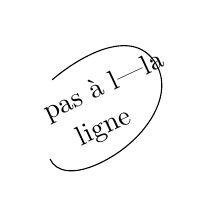
\begin{tikzpicture}[x=0.45cm,y=0.45cm]\draw[rotate=25] (-1,1.3) .. controls (.3,1.65) and (1.8,1.6) .. (1.85,.4) .. controls (1.9,-.6) and (.6,-1.4) .. (-.8,-1.4) .. controls (-1.6,-1.4) and (-2,-1.1) .. (-2,-.7);\node[rotate=25] at (0,0.55) {pas à \unsure{l|la}};\node[rotate=25] at (0,-0.6) {ligne};\end{tikzpicture}}}}
\margin{\figure{\handwritten{
\begin{tikzpicture}[x=0.3cm,y=0.3cm]\draw (1,.8) .. controls (.3,1.25) and (-.7,1.1) .. (-.8,.45);\draw (-.8,.25) .. controls (-.4,.05) and (.4,.1) .. (1.15,.3);\end{tikzpicture}}}}
Posons alors $W=V\handwritten{\cap}I$, c'est un espace vectoriel sur $k$ de dimension finie, dont nous noterons $d$ la dimension. Puisque $V$ contient tous les $g_i$, $W$ engendre \deleted{l'algèbre}\inserted{\handwritten{l'ideal}} $I$.

\margin{\figure{\handwritten{
\begin{tikzpicture}[x=0.3cm,y=0.3cm]\draw (1,.8) .. controls (.3,1.25) and (-.7,1.1) .. (-.8,.45);\draw (-.8,.25) .. controls (-.4,.05) and (.4,.1) .. (1.15,.3);\end{tikzpicture}}}}
Notons $p:A\handwritten{\longrightarrow}A/I=B$ l'application canonique, et $q=p\handwritten{\otimes}\operatorname{id}_A:A\handwritten{\otimes}_k A\handwritten{\longrightarrow}(A/I)\handwritten{\otimes}_k A$ Alors l'action de $H$ sur $A$ est déterminée par $q\mathbin{o}\handwritten{\Delta}:A\handwritten{\longrightarrow}B\handwritten{\otimes}_k A$. Puisque $H$ est un sous-préschéma en groupes de $G$, l'application diagonale $A/I\handwritten{\longrightarrow}(A/I)\handwritten{\otimes}_k(A/I)=((A/I)\handwritten{\otimes}_k A)/((A/I)\handwritten{\otimes}_k I)$ se déduit de $q\mathbin{o}\handwritten{\Delta}$ par passage au quotient, ce qui montre que $(q\mathbin{o}\handwritten{\Delta})(I)\subset(A/I)\handwritten{\otimes}_k I$, autre-\linebreak ment dit, $I$ est stable sous $H$. Puisque $V$ est stable sous $G$, donc sous $H$, on voit que $W$ est stable sous $H$.

Posons $E=\handwritten{\wedge}^d V$, soit $(w_1,\ldots,w_d)$ une base de $W$ sur $k$, et soit $(e_{\unsure{o|0}},\mathinner{..},e_n)$ une base de $E$ sur $k$ contenant $e_{\unsure{o|0}}=w_1\handwritten{\wedge}\cdots\handwritten{\wedge}w_d$. L'opération de $G$ sur $\handwritten{V}$ détermine canoniquement une opération de $G$ sur $\handwritten{\wedge}^d V$, qui définit une application linéaire $\handwritten{\rho}:E\handwritten{\longrightarrow}A\handwritten{\otimes}_k E$. Posons $\handwritten{\rho}(e_i)=\handwritten{\sum}a_j^i\handwritten{\otimes}e_j$, et $a_i=a_i^{\unsure{o|0}}$. Puisque $W$ est stable sous $H$, si on pose \margin{\figure{\begin{tikzpicture}[x=1cm,y=1cm]\draw[thin] (0,.02)--(.18,-.01);\end{tikzpicture}}}$\handwritten{\sigma}=(p\handwritten{\otimes}\operatorname{id}_E)\mathbin{o}\handwritten{\rho}:E\handwritten{\longrightarrow}(A/I)\handwritten{\otimes}_k E$, il est clair que $\handwritten{\sigma}(e_{\unsure{o|0}})$ est proportionnel à $e_{\unsure{o|0}}$, autrement dit, pour $1\leqq i\leqq n$, on a $a_i\in I$. L'axio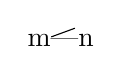
\begin{tikzpicture}[x=1cm,y=1cm,baseline=(a.base)]\node[inner sep=0pt] (a) at (0,0) {\unsure{m|n}};\draw (-.12,.05)--(.18,.16);\end{tikzpicture}e (CM1) de (\deleted{Exp.} I 4.7.2) appliqué à
